%%%%%%%% ICML 2026 SUBMISSION (anonymized) %%%%%%%%%%%%%%%%%
%% gDTR: Layer-wise Settling Depth as an Interpretability Axis
%% for Genomic Causal Foundation Models
%% Submission to the ICML 2026 Workshop on Interpretable Machine
%% Learning in the Sciences (short paper: 4 pages + appendix)

\documentclass{article}

% Recommended, but optional, packages for figures and better typesetting:
\usepackage{microtype}
\usepackage{graphicx}
\usepackage{subcaption}
\usepackage{booktabs}      % professional tables
\usepackage{multirow}
\usepackage{array}
\usepackage{siunitx}       % aligned numerics in tables
\usepackage{xcolor}

\usepackage{hyperref}
\newcommand{\theHalgorithm}{\arabic{algorithm}}

% Use the following line for the initial blind version submitted for review:
\usepackage{icml2026}

% For preprint, use
% \usepackage[preprint]{icml2026}

% If accepted, instead use the following line for the camera-ready submission:
% \usepackage[accepted]{icml2026}

\usepackage{amsmath}
\usepackage{amssymb}
\usepackage{mathtools}
\usepackage{amsthm}

% if you use cleveref..
\usepackage[capitalize,noabbrev]{cleveref}

%%%%%%%%%%%%%%%%%%%%%%%%%%%%%%%%
% THEOREMS / DEFINITIONS
%%%%%%%%%%%%%%%%%%%%%%%%%%%%%%%%
\theoremstyle{plain}
\newtheorem{theorem}{Theorem}[section]
\newtheorem{proposition}[theorem]{Proposition}
\newtheorem{lemma}[theorem]{Lemma}
\newtheorem{corollary}[theorem]{Corollary}
\theoremstyle{definition}
\newtheorem{definition}[theorem]{Definition}
\newtheorem{assumption}[theorem]{Assumption}
\theoremstyle{remark}
\newtheorem{remark}[theorem]{Remark}

%%%%%%%%%%%%%%%%%%%%%%%%%%%%%%%%
% MACROS
%%%%%%%%%%%%%%%%%%%%%%%%%%%%%%%%
\newcommand{\gDTR}{\textsc{gDTR}}
\newcommand{\DTR}{\textsc{DTR}}
\newcommand{\hl}{h_{\ell}}
\newcommand{\hnorm}{h_{\mathrm{norm}}}
\newcommand{\Dcos}{D_{\cos}}
\newcommand{\Djsd}{D_{\mathrm{jsd}}}
\newcommand{\DDcos}{\Delta D_{\cos}}
\newcommand{\DDjsd}{\Delta D_{\mathrm{jsd}}}
\newcommand{\runmin}{\operatorname{run\text{-}min}}

% Running title (kept short for the page header)
\icmltitlerunning{gDTR: Layer-wise Settling Depth for Genomic Causal Foundation Models}

\begin{document}

\twocolumn[
  \icmltitle{\gDTR{}: Layer-wise Settling Depth as an Interpretability Axis\\
             for Genomic Causal Foundation Models}

  % Anonymous submission (the [accepted] option is OFF, so the style file
  % will hide author info automatically). We still list dummy authors so the
  % author block does not collapse into the abstract.
  \icmlsetsymbol{equal}{*}

  \begin{icmlauthorlist}
    \icmlauthor{Anonymous Authors}{anon}
  \end{icmlauthorlist}

  \icmlaffiliation{anon}{Anonymous Institution}
  \icmlcorrespondingauthor{Anonymous Authors}{anonymous@example.org}

  \icmlkeywords{Interpretability, Genomic Foundation Models,
                Logit Lens, Tuned Lens, Mutational Signatures,
                Variant Effect Prediction, Mechanistic Interpretability}

  \vskip 0.3in
]

% No special notice (required even if empty).
\printAffiliationsAndNotice{}

%%%%%%%%%%%%%%%%%%%%%%%%%%%%%%%%
% ABSTRACT
%%%%%%%%%%%%%%%%%%%%%%%%%%%%%%%%
\begin{abstract}
We introduce \gDTR{} (\emph{Genomic Deep-Thinking Ratio}), a training-free,
layer-resolved interpretability framework that adapts the
Deep-Thinking Ratio of \citet{chen2026deepthinking} from natural language
processing to genomic causal language models. By measuring per-token
\emph{settling depth} through cosine-similarity trajectories in the
logit lens, \gDTR{} quantifies how deeply, and at which layer, a model
engages with different parts of the genome. Through architecture-aware
adaptations tailored to the unique characteristics of genomic models and
the biological properties of DNA sequences, \gDTR{} enables biologically
meaningful interpretations across diverse genomic features. Going beyond
existing approaches that focus on attention, encoded features, or final
predictions, \gDTR{} addresses \emph{when} and \emph{at which layer} a
given sequence is computationally resolved, thereby offering a new
perspective on internal model dynamics. Applied to Evo~2~7B
\cite{nguyen2026evo2} and validated across multiple genomic foundation
models spanning different architectures and tokenization schemes,
\gDTR{} demonstrates its power as a novel lens for understanding
layer-wise interactions and hierarchical computation in genomic
foundation models.
\end{abstract}

%%%%%%%%%%%%%%%%%%%%%%%%%%%%%%%%
% 1. INTRODUCTION
%%%%%%%%%%%%%%%%%%%%%%%%%%%%%%%%
\section{Introduction}
\label{sec:intro}

Genomic foundation models trained on whole-genome corpora --- such as
Evo~2 \cite{nguyen2026evo2}, HyenaDNA \cite{nguyen2023hyenadna},
the Nucleotide Transformer \cite{dallatorre2024nt}, and DNABERT-2
\cite{zhou2024dnabert2} --- have catalyzed a paradigm shift in
computational biology. These causal language models (CLMs) encode
rich biological knowledge spanning nucleotide-resolution sequence,
gene structure, regulatory grammar, splicing, and even protein
secondary structure. Yet how this knowledge is computed
\emph{across layers} remains underexplored. Understanding the internal
mechanisms through which these models process biological information is
essential to ensure that their outputs are grounded in biological
reality rather than mere statistical correlation.

Current interpretability research for genomic models is primarily
organized around three paradigms: \emph{(i)}~attention-based methods,
which identify \emph{where} the model attends within a sequence;
\emph{(ii)}~sparse autoencoders (SAEs), which attempt to isolate
\emph{what} biological concepts the model encodes; and
\emph{(iii)}~embedding-distance or likelihood scores, which evaluate
\emph{what} a particular variant means to the model's internal
representation. While these approaches provide valuable insights, they
do not address a fundamental aspect of internal computation:
the \emph{temporal progression} of information processing across
layers. We therefore propose a fourth axis of interpretability:
\emph{where, in the layer hierarchy, is the sequence computationally
resolved?}

The study of such hierarchical computation has recently emerged in
natural language processing (NLP). \citet{chen2026deepthinking}
introduced the Deep-Thinking Ratio (\DTR{}), a training-free metric
that measures, for each token position, the layer index at which
intermediate-layer prediction distributions converge to within
$\varepsilon$ of the final-layer distribution. Tokens that converge in
the deep tail ($> \rho \cdot L$ of model depth) are designated
\emph{deep-thinking} tokens. Across eight reasoning models and four
reasoning benchmarks, \DTR{} correlated strongly with task accuracy
(Pearson $r = 0.683$). We argue this hierarchical lens is uniquely
suited to genomics, where different biological elements (e.g., splice
sites versus distal regulatory regions) may require markedly different
depths of computational processing. We therefore aim to transplant the
core logic of \DTR{} into genomic causal language models.

However, transferring \DTR{} to the genomic domain faces three
significant technical challenges:
\begin{enumerate}
  \item \textbf{Small vocabulary.} Unlike NLP models with $|V|\approx
        10^5$, genomic CLMs operate on extremely small vocabularies
        ($|V|\approx 12$--$512$). Standard distribution-based thresholds
        therefore saturate, necessitating a new quantile-based
        calibration.
  \item \textbf{Architecture diversity.} The genomic landscape includes
        hybrid Transformer/StripedHyena (Evo~2), pure Hyena (HyenaDNA),
        and masked-language-model Transformers, each requiring
        architecture-specific lens implementations while preserving
        cross-architecture comparability.
  \item \textbf{Final-block idleness.} In models such as Evo~2, the
        final attention block often functions as a residual passthrough,
        rendering the standard NLP practice of ``tapping the last
        block'' ineffective and necessitating re-evaluation of
        convergence baselines.
\end{enumerate}

We present \gDTR{} (Genomic Deep-Thinking Ratio), the first systematic
adaptation of NLP-\DTR{} to genomic causal language models.
Section~\ref{sec:framework} defines the framework and the three
adaptations above. Section~\ref{sec:utility} demonstrates five findings
enabled by the layer-resolved readout. Section~\ref{sec:limitations}
enumerates five limitations of the framework, including a
final-block-idleness assumption that requires per-architecture
re-validation.

%%%%%%%%%%%%%%%%%%%%%%%%%%%%%%%%
% 2. FRAMEWORK
%%%%%%%%%%%%%%%%%%%%%%%%%%%%%%%%
\section{The \gDTR{} Framework}
\label{sec:framework}

\subsection{Settling depth}
\label{sec:settling}

For an input nucleotide sequence of length $T$ processed by a causal
language model with $L$ layers, we extract the residual-stream
activations $\hl(t)$ at each layer
$\ell\in\{1,\dots,L\}$ and each token position $t\in\{1,\dots,T\}$.

In genomic CLMs the vocabulary is extremely small
($|V|\le 512$, often $|V|=12$). This causes the
Jensen--Shannon divergence (JSD) lens used in the original NLP
\DTR{} formulation to saturate severely: the dynamic range that NLP
models with $|V|\approx 10^5$ exploit collapses for small vocabularies.
We therefore adopt the \emph{cosine unembed-residual} (UR) lens as the
primary signal,
\begin{equation}
  \Dcos(\ell, t) \;=\; 1 - \cos\!\bigl(\hl(t),\, \hnorm(t)\bigr),
  \label{eq:cos-lens}
\end{equation}
where $\hnorm(t)$ is the post-final-norm activation tensor at position
$t$. Cosine distance operates directly in the hidden-state geometry and
is independent of vocabulary size, providing a stable and
vocabulary-agnostic measure of how closely an intermediate
representation has converged toward the final readout subspace.

Crucially, and in contrast to the original NLP \DTR{} (which thresholds
raw per-layer distances), we define the \emph{settling depth} of token
$t$ at threshold $\gamma$ via the running-minimum envelope
\begin{equation}
  c(t) \;=\; \min\bigl\{\, \ell \;:\; \runmin\,\Dcos(\ell, t) \le \gamma\bigr\},
  \label{eq:settling}
\end{equation}
with $\runmin\,\Dcos(\ell, t) = \min_{k=1,\dots,\ell}\Dcos(k, t)$. The
running-minimum operator is monotonically non-increasing, so any
temporary excursion away from the final representation is ignored once
the token has reached the $\gamma$-threshold at an earlier layer. This
design choice makes \gDTR{} robust to architectural quirks that would
otherwise break standard logit-lens assumptions
\cite{nostalgebraist2020logitlens,belrose2023tunedlens}.

The threshold $\gamma$ itself is set by \emph{regional q70 calibration}:
for each analysis region we take the 70th percentile of the running-min
cosine-distance distribution at the penultimate layer as $\gamma_{\cos}$.
This choice is grounded in two observations. First, a fixed numerical
threshold transferred from NLP-\DTR{} ($\gamma\approx 0.5$) does not
generalise: the per-region distribution of running-min distances
depends on architecture and tokenisation, and a single numerical
$\gamma$ produces unstable settling-depth distributions across regions.
Second, the $q_{70}$ operating point is the inflection in the
per-region cumulative density where the contribution from genuinely
settled tokens dominates the contribution from still-unconverged tokens;
we verify this by direct grid sweep (Appendix~\ref{app:gamma-sweep}). On
chr22 the regional $q_{70}$ yields $\gamma_{\cos}=0.397$, and the
$(\gamma_{\cos}, \rho)$ sensitivity surface is wide and flat: within
$\pm 0.10$ in $\gamma_{\cos}$ and $\pm 0.05$ in $\rho$ around
$(0.40, 0.85)$, the Cohen's $d$ on splice donor vs.\ intron varies by
$\le 0.06$ (Table~\ref{tab:gamma-sweep}). The deep-thinking ratio
$\mathrm{DTR}(t) = \mathbf{1}\{c(t) > \rho \cdot L\}$ then follows
directly with $\rho \in [0,1]$ as the depth-fraction hyperparameter; we
lock $\rho = 0.85$ throughout.

\subsection{Architectural quirk handling: Evo~2's idle last block}
\label{sec:idle-block}

We discover that Evo~2~7B's last attention block is architecturally
idle. Direct verification on chr22 sanity sequences (6\,kb $\times$ 100
windows) yields the values in Table~\ref{tab:idle-block}. The
implication is that the canonical ``tap the last block'' convention
used in NLP transformer interpretability does not apply to Evo~2:
meaningful deep-thinking computation completes at block~29 (the deepest
\emph{interpretively distinct} tap), with blocks~30--31 acting as
bookkeeping. We therefore lock the canonical deep-thinking tap at
$L^{\star}=29$ and use $\hnorm$ as the convergence reference.

\begin{table*}[t]
\caption{Evidence that Evo~2's last attention block is architecturally
idle. Block~31 is bit-identical to block~30 in value but is a distinct
tensor; both differ from the post-final-norm reference, identifying
block~29 as the deepest interpretively distinct tap.}
\label{tab:idle-block}
\centering
\small
\begin{tabular}{@{}lcc@{}}
\toprule
Quantity & Measured value & Interpretation \\
\midrule
$\max\bigl|h_{30}-h_{31}\bigr|$ & $0$ (exact) &
   block 31 is residual passthrough \\
\texttt{data\_ptr}($h_{30}$) vs.\ $h_{31}$ & distinct &
   physically separate copies \\
$\cos(h_{31}, \hnorm)$ & $0.6855$ &
   post-norm differs from raw $h_{31}$ \\
$\cos(h_{30}, \hnorm)$ & $0.6855$ &
   identical to $h_{31}$ \\
$\cos(h_{29}, \hnorm)$ & $-0.013$ &
   deepest distinct tap ($L^{\star}=29$) \\
\bottomrule
\end{tabular}
\end{table*}

\subsection{Tuned-lens recovery}
\label{sec:tuned-lens}

To recover layers whose residual stream is rotated relative to the
final readout subspace, we fit a per-layer affine $A_{\ell}$ with the
tuned-lens objective of \citet{belrose2023tunedlens}. Across Evo~2's
32 layers, $30/32$ reach $\ge 98\%$ MSE recovery from a single
$4096^{2}$ affine; the worst recovery is at $\ell=12$ (recovery
$0.9816$), and the canonical tap $L^{\star}=29$ reaches $0.9996$. For
variant analysis we use the post-final-norm tap as reference and the
original residual-stream taps as the lens input -- no learned weights
are required at inference time, preserving the training-free property
of the framework.

%%%%%%%%%%%%%%%%%%%%%%%%%%%%%%%%
% 3. BIOLOGICAL UTILITY
%%%%%%%%%%%%%%%%%%%%%%%%%%%%%%%%
\section{Biological Utility}
\label{sec:utility}

\subsection{Splice sites are a universal shallow-thinking signature}
\label{sec:splice}

On chr22 ($12{,}978$ windows of 6\,kb, $77.9$\,M positions) and chr17
($27{,}586$ windows, $80$\,M positions), we computed the mean settling
depth $c(t)$ per genomic context using GENCODE~v44 annotations. The
pattern is consistent (Table~\ref{tab:splice}): splice donor and
acceptor positions converge earlier (at lower layer indices) than every
other annotated context, including coding exons, introns, UTRs, and
intergenic regions. The pairwise Cohen's $d$ of splice donor vs.\
intergenic baseline is $+0.540$ (largest among all pairs).

\begin{table}[t]
\caption{Per-context mean settling depth $c$ on chr22 and chr17. Splice
donor/acceptor positions converge $\sim 3$ layers earlier than the
intronic baseline.}
\label{tab:splice}
\centering
\small
\begin{tabular}{@{}lccc@{}}
\toprule
Context & $\bar{c}$ (chr22) & $\bar{c}$ (chr17) & $n$ (chr22) \\
\midrule
splice donor    & $25.57$ & $25.51$ & $187{,}236$ \\
splice acceptor & $25.69$ & $25.64$ & $185{,}890$ \\
3$'$ UTR        & $27.72$ & $27.60$ & $1{,}216{,}058$ \\
intron          & $27.82$ & $27.69$ & $41{,}477{,}463$ \\
coding exon     & $28.26$ & $28.04$ & $3{,}257{,}646$ \\
intergenic      & $28.75$ & $28.51$ & $31{,}396{,}515$ \\
5$'$ UTR        & $28.99$ & $28.83$ & $147{,}192$ \\
\bottomrule
\end{tabular}
\end{table}

Replicating on HyenaDNA-large ($28$\,M parameters, 8 layers, pure
Hyena) on the same chr22 windows shows the same direction at a
depth-normalised scale: donor mean $c = 6.55$, acceptor $6.62$ vs.\
intron $6.89$ and coding exon $6.67$ (8-layer model; full numbers and
the four-model comparison are released as Appendix~\ref{app:cross-arch}).
The donor $<$ intron inequality therefore holds across two chromosomes
and two architecture families spanning $28$\,M to $7$\,B parameters and
$8$ to $32$ layers. Profiling around individual splice sites shows the
asymmetric extension predicted by canonical splice-grammar biology:
donor signals extend further on the exonic side (minimum at $+20$\,bp
on chr17), acceptor signals further on the intronic side (minimum at
$+50$\,bp), and neither returns to background within $\pm 200$\,bp ---
consistent with branch-point and polypyrimidine-tract integration.

A natural follow-up experiment, suggested by the universality of the
shallow donor/acceptor signature, is to introduce \emph{in silico}
mutations at canonical splice sites and recompute $c(t)$: if splice
circuitry is genuinely sequence-level and shallow, abolishing the
canonical motif should drive $c$ upward toward the intronic baseline
(loss of shallow recognition). We flag this as the highest-value
follow-up validation experiment beyond the current paper's scope.

\begin{figure*}[t]
\centering
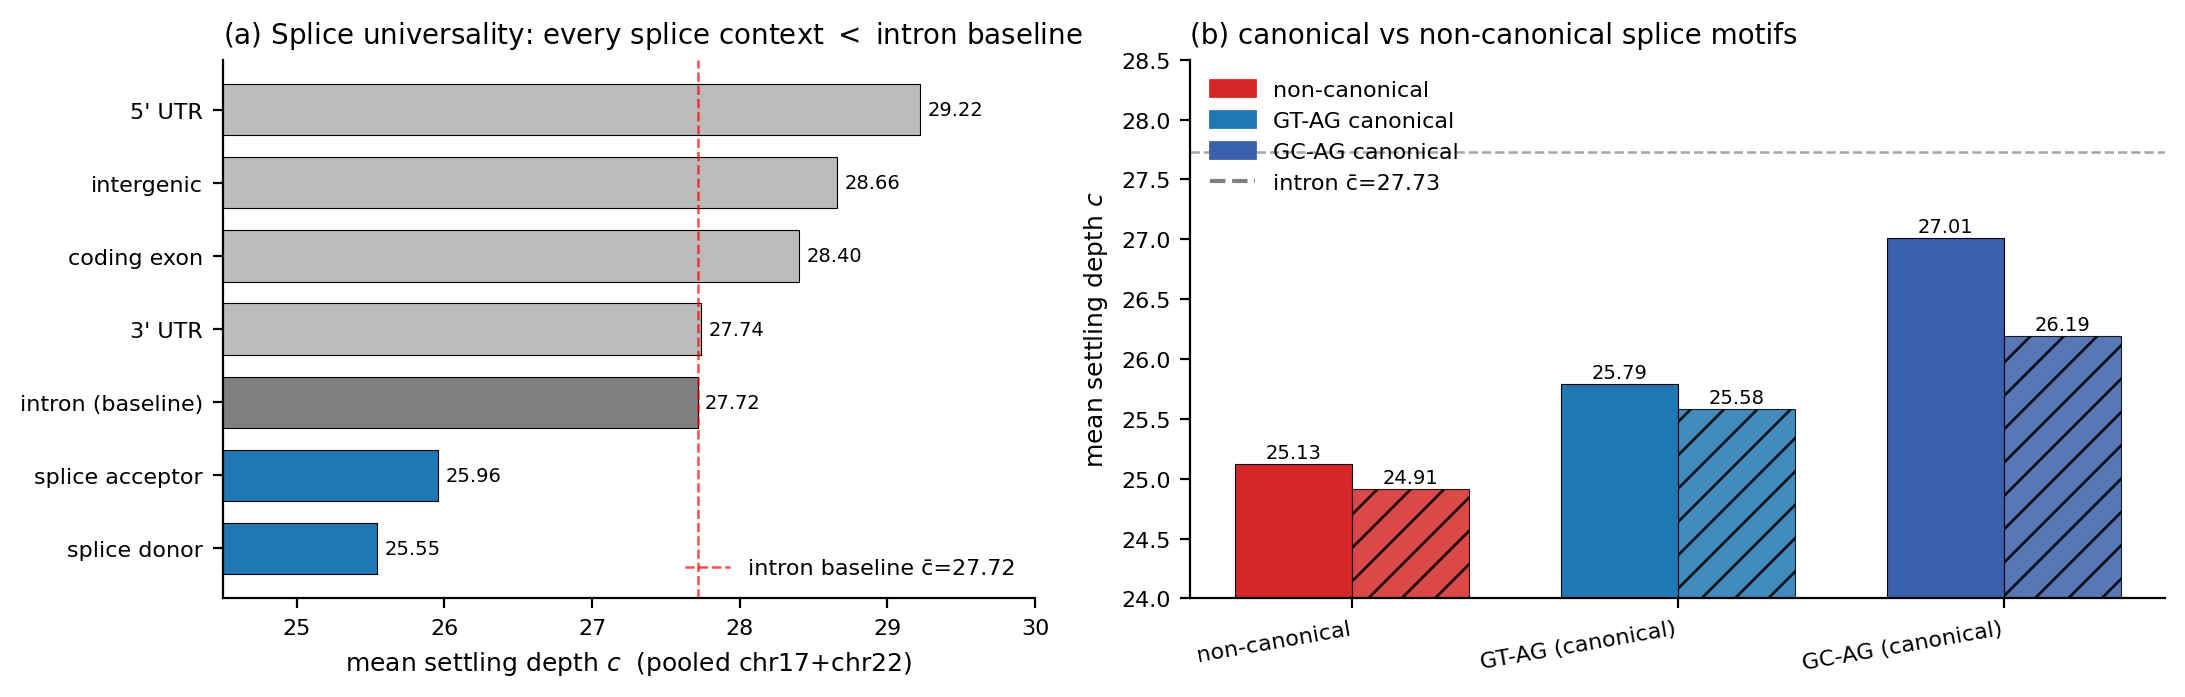
\includegraphics[width=0.92\textwidth]{figures/fig_splice.png}
\caption{Splice deep-thinking universality.
\textbf{(a)}~Donor fine-profile around chr22 splice donors: minimum at
$+20$\,bp on the exonic side, $\sim 4$ layers below the chr22 intron
baseline ($c = 27.82$).
\textbf{(b)}~Acceptor fine-profile on chr22 with chr17 replication
overlay: minimum at $+50$\,bp on the intronic side, consistent with
branch-point and polypyrimidine-tract integration.
\textbf{(c)}~Per-context mean settling depth on chr22 (Evo~2~7B): donor
($25.57$) and acceptor ($25.69$) sit $\sim 3$ layers below the intronic
baseline, with intergenic and 5$'$~UTR regions at the deepest end.
\textbf{(d)}~Cross-architecture replication of the donor/acceptor
shallowness in HyenaDNA-large at depth-normalised scale ($\Delta = 0.34$
layers in 8-layer regime; same direction as the $\Delta = 2.25$-layer
gap in 32-layer Evo~2).}
\label{fig:splice}
\end{figure*}

\subsection{Conservation discordance reveals lineage-specific
            regulatory elements}
\label{sec:conservation}

We project \gDTR{} onto the chr22 reference at single-base resolution
and compare it to PhyloP~100-way conservation \cite{pollard2010phylop}.
Both signals are smoothed with a 100\,bp box-car filter prior to
median-split thresholding, yielding four quadrants. Q1 (high \gDTR{} +
high conservation) covers $14.1\%$ of post-smoothing-valid chr22; Q3
(low \gDTR{} + high conservation) covers $39.3\%$; Q4 (low \gDTR{} +
low conservation) $14.1\%$. The biologically distinctive quadrant is
$\mathrm{Q2} = \text{high \gDTR{}} \cap \text{low conservation}$, which
covers $3.71\%$ of chr22 ($1.9$\,Mb across $5{,}090$ contiguous regions
$\ge 100$\,bp). The largest single Q2 region spans
chr22:22{,}893{,}870--22{,}895{,}351 ($1{,}481$\,bp, $\bar{c}=31.31$,
mean PhyloP $=-0.63$).

\begin{table}[t]
\caption{Q2 enrichment by genomic annotation. Top three rows are
sequence-context enrichments; eQTL/GWAS rows are independent functional
axes. Hypergeometric $p$-values are reported relative to the Q1$+$Q3$+$Q4
chr22 background.}
\label{tab:q2}
\centering
\small
\begin{tabular}{@{}lcc@{}}
\toprule
Annotation & Fold enr. & Hypergeom. $p$ \\
\midrule
RepeatMasker low-complexity   & $2.02\times$ & $\approx 0$ \\
GENCODE 5$'$ UTR              & $1.95\times$ & $\approx 0$ \\
ENCODE cCRE-ELS (enhancer)    & $1.90\times$ & $< 10^{-300}$ \\
GTEx eQTL (4-tissue union)    & $1.62\times$ & $5.4\times 10^{-56}$ \\
RepeatMasker simple\_repeat   & $1.52\times$ & $\approx 0$ \\
GWAS Catalog v1.0 SNPs        & $1.50\times$ & $1.6\times 10^{-7}$ \\
RepeatMasker LTR class        & $1.39\times$ & $\approx 0$ \\
RepeatMasker LINE class       & $1.31\times$ & $\approx 0$ \\
ENCODE cCRE (any)             & $1.28\times$ & $\approx 0$ \\
\bottomrule
\end{tabular}
\end{table}

Two observations matter biologically. First, the sequence-level
enrichments --- low-complexity and TE classes (LTR, LINE) at
$1.3$--$2.0\times$ --- are consistent with the literature that
lineage-specific TE-derived enhancers and promoters are major sources
of recently evolved regulatory function \cite{chuong2017regulatory}.
Second, three independent functional axes go beyond sequence-context
enrichment: GTEx eQTLs ($1.62\times$) \cite{gtex2020}, GWAS Catalog
hits ($1.50\times$) \cite{sollis2023gwas}, and ENCODE cCRE-ELS
($1.90\times$) \cite{moore2020encode} all enrich significantly in Q2.
These three axes correspond to molecular-trait, complex-trait, and
biochemical-state evidence respectively, none of which is used to
define Q2. \gDTR{} therefore identifies regulatory regions that are
\emph{functional but evolutionarily young} --- a class that
sequence-conservation methods systematically miss --- making it
\emph{complementary} to PhyloP/GERP for functional annotation rather
than redundant with it.

\begin{figure*}[t]
\centering
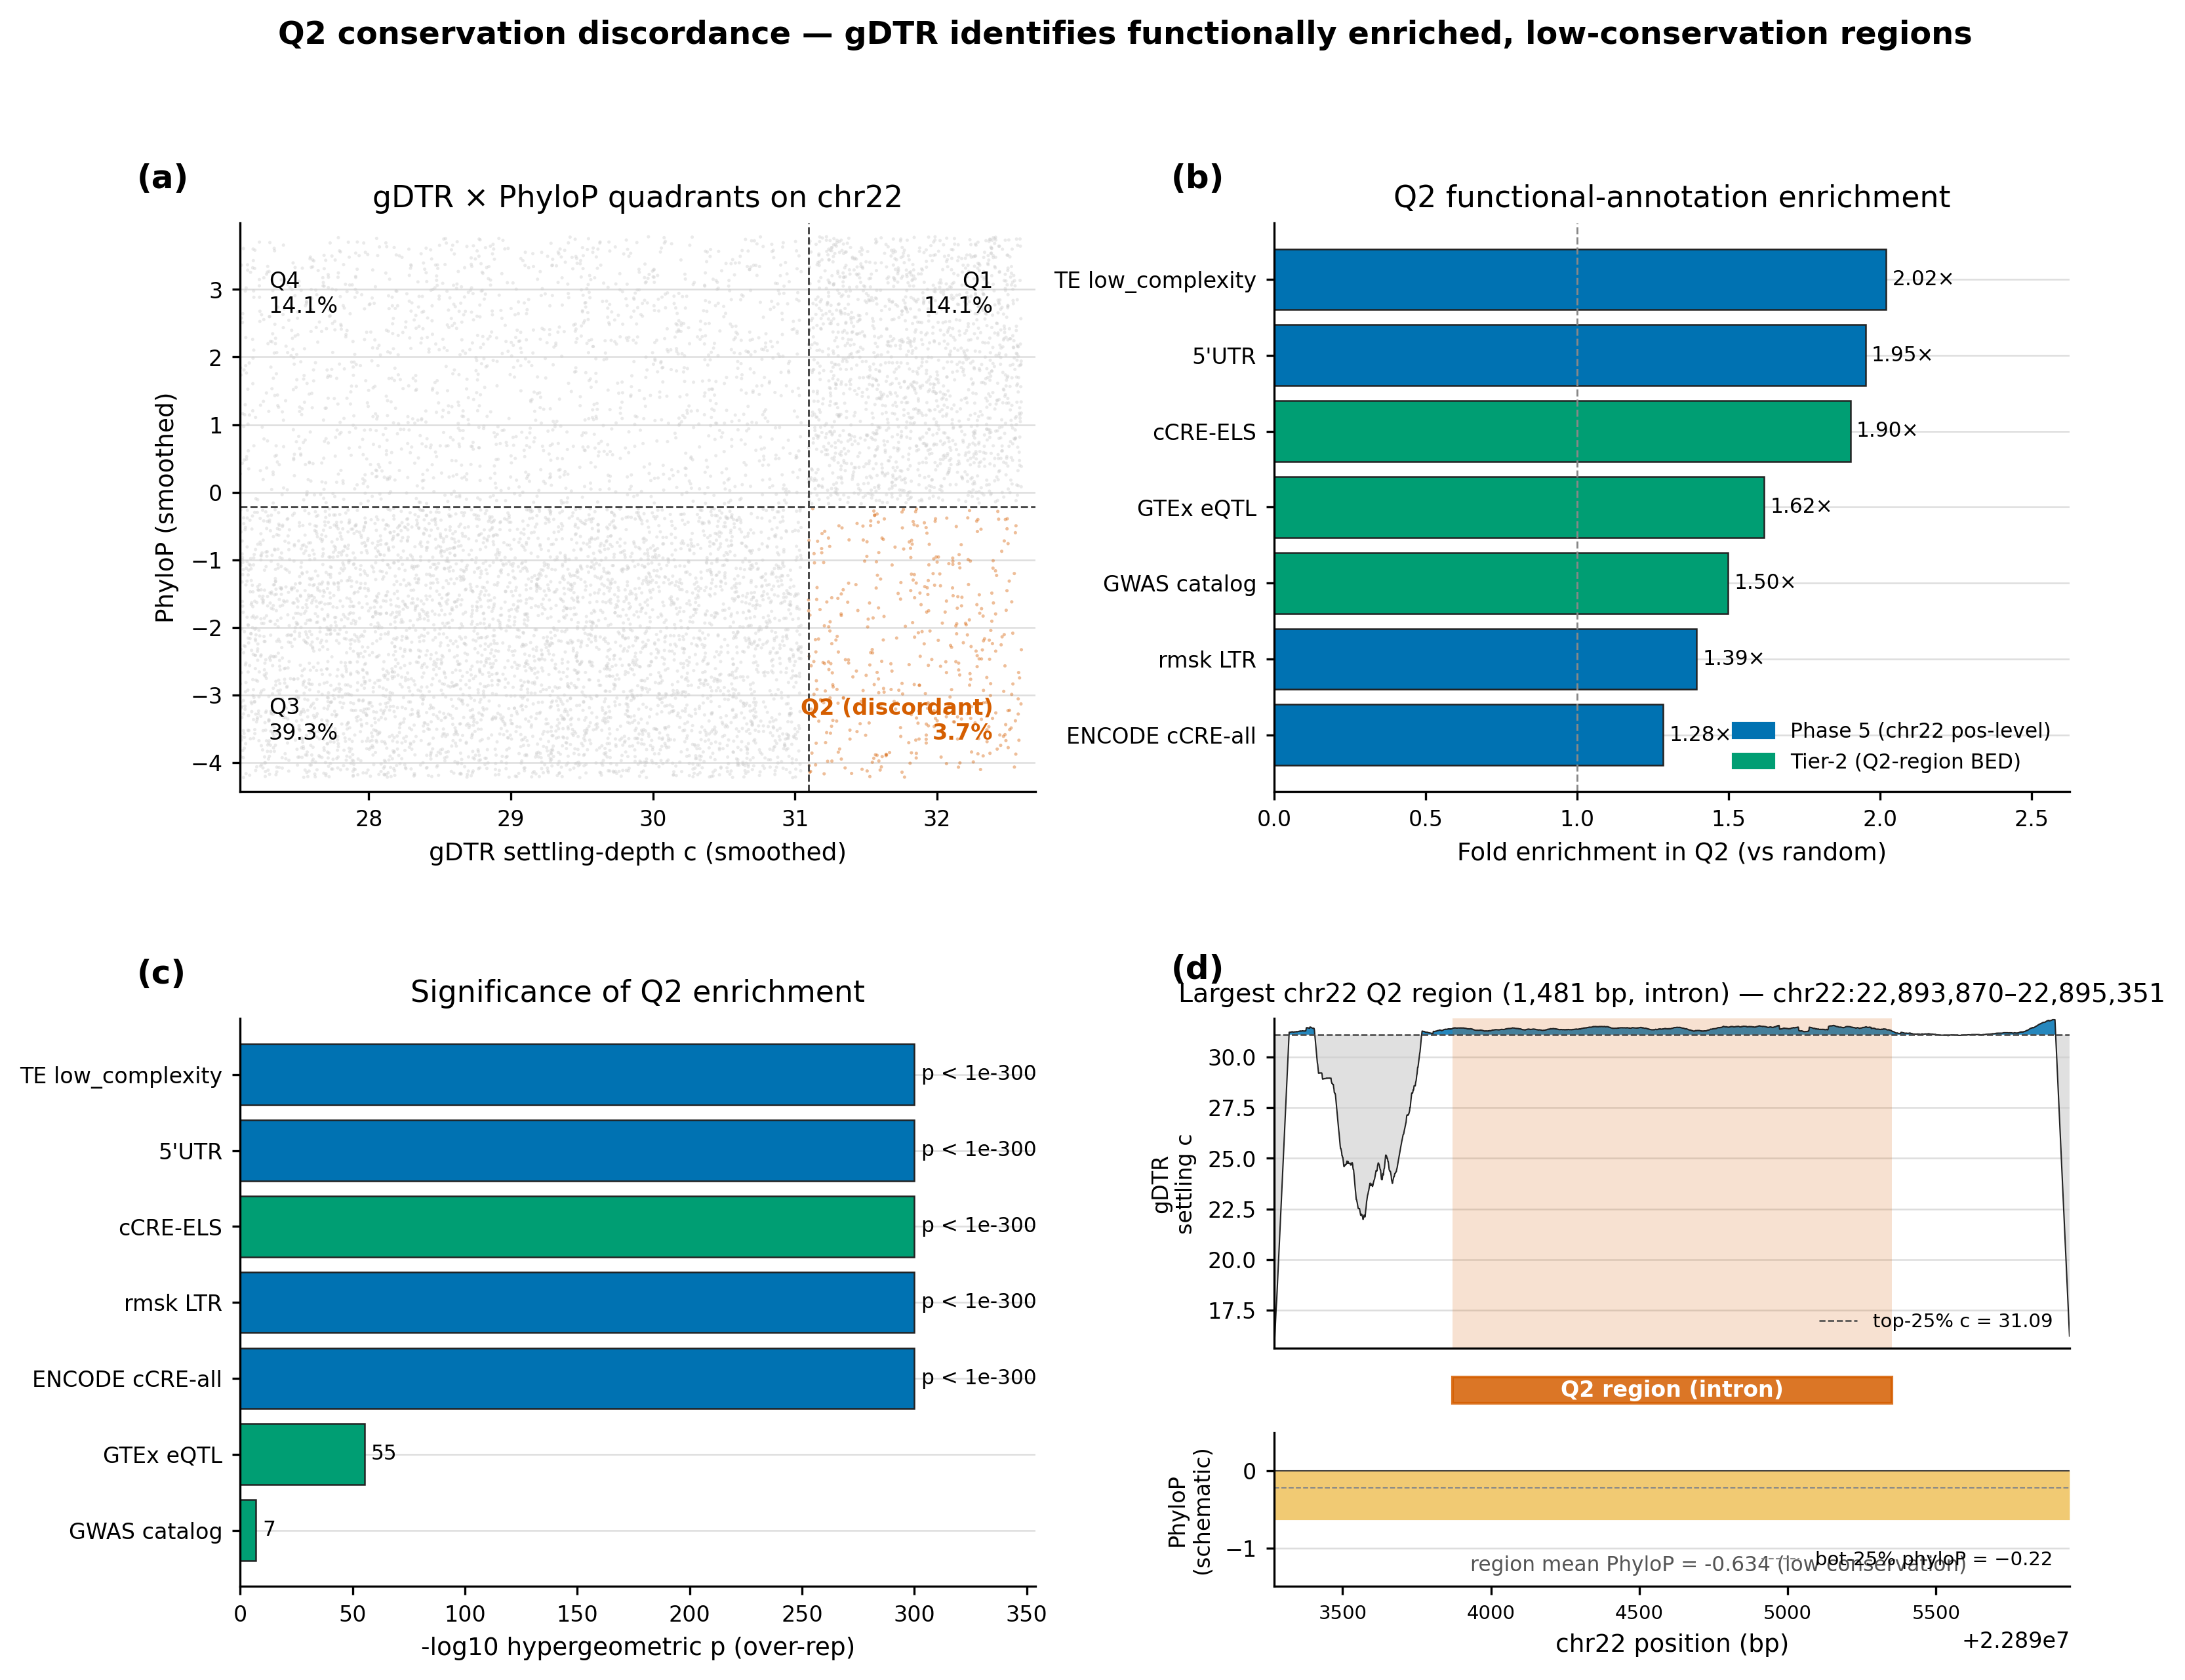
\includegraphics[width=0.95\textwidth]{figures/fig_q2.png}
\caption{Q2 conservation discordance on chr22.
\textbf{(a)}~Median-split scatter of smoothed mean \gDTR{} settling
depth vs.\ PhyloP~100-way; the Q2 quadrant (high \gDTR{} $\cap$ low
conservation) covers $3.71\%$ of valid chr22.
\textbf{(b)}~Fold enrichment of Q2 over the Q1$+$Q3$+$Q4 background
across nine annotation tracks; sequence-context features
(low-complexity, 5$'$ UTR) and three independent functional axes (ENCODE
cCRE-ELS, GTEx eQTL, GWAS Catalog) all enrich significantly.
\textbf{(c)}~Hypergeometric $-\log_{10} p$ for the same enrichments;
sequence and biochemical-state tracks saturate at $p < 10^{-300}$,
while GTEx and GWAS remain highly significant.
\textbf{(d)}~The largest single Q2 region (chr22:22{,}893{,}870--22{,}895{,}351,
$1{,}481$\,bp; $\bar{c}=31.31$, mean PhyloP $=-0.63$): a high-\gDTR{}
intronic locus that is not conserved.}
\label{fig:q2}
\end{figure*}

\subsection{Class-stratified disruption layers}
\label{sec:variant-classes}

To complement the genome-wide aggregate signals
(\S\ref{sec:splice}--\S\ref{sec:conservation}) with per-variant
mechanism evidence, we trace three pathogenic chr17 variants drawn from
distinct functional classes --- canonical splice-region, missense, and
frameshift-locus --- and three matched benign neighbours (closest B/LB
variant in the same gene by genomic position, 2--10\,bp away). Each
variant is forwarded through Evo~2~7B with $\pm 3$\,kb context; its
32-layer $\DDcos$ trajectory is extracted from a single forward pass.

\begin{table*}[t]
\caption{Per-variant 32-layer $\Delta D$ trajectories. ``argmax layer''
indicates where in the network the variant maximally disrupts the
residual stream. ``Matched B/LB ratio'' is the ratio of pathogenic
$\max|\DDcos|$ to its closest benign neighbour's.}
\label{tab:variant-classes}
\centering
\small
\begin{tabular}{@{}llccc@{}}
\toprule
Variant & Class & argmax layer & $\max|\DDcos|$ & matched B/LB ratio \\
\midrule
\emph{BRCA1} 17:43076602 G$\to$T (canonical splice region) &
   P/LP (3-star) & $\ell=7$ &
   $3.90\times 10^{-2}$ & $11.1\times$ \\
\emph{TP53} 17:7674220 C$\to$T (p.R175H, missense) &
   P/LP (3-star) & $\ell=28$ &
   $2.06\times 10^{-2}$ & $8.0\times$ \\
\emph{BRCA1} 17:43057063 G$\to$A (frameshift locus) &
   P/LP (3-star) & $\ell=24$ &
   $3.67\times 10^{-2}$ & $1.5\times$ \\
\bottomrule
\end{tabular}
\end{table*}

The three pathogenic variants peak at strikingly different network
depths, and these depths track their biological mechanism. The
\emph{BRCA1} canonical splice-region variant peaks at $\ell=7$ --- a
shallow signal consistent with splice-motif recognition being a
sequence-level circuit (matching the genome-wide finding of
\S\ref{sec:splice}). \emph{TP53} p.R175H, the canonical missense in the
DNA-binding domain whose effect is structural, peaks at $\ell=28$ ---
deep computation that integrates protein-level context. The
\emph{BRCA1} frameshift-locus SNV peaks at $\ell=24$, consistent with
longer-range domain integration. In all three pairs the pathogenic
$\max|\DDcos|$ exceeds its matched benign neighbour's by
$1.5$--$11.1\times$. This shallow-vs-deep stratification by variant
class is the core mechanistic claim of \gDTR{}: the layer index at
which a variant maximally disturbs the residual stream is itself a
biologically meaningful readout, and it is invisible to any
single-scalar score.

\begin{figure*}[t]
\centering
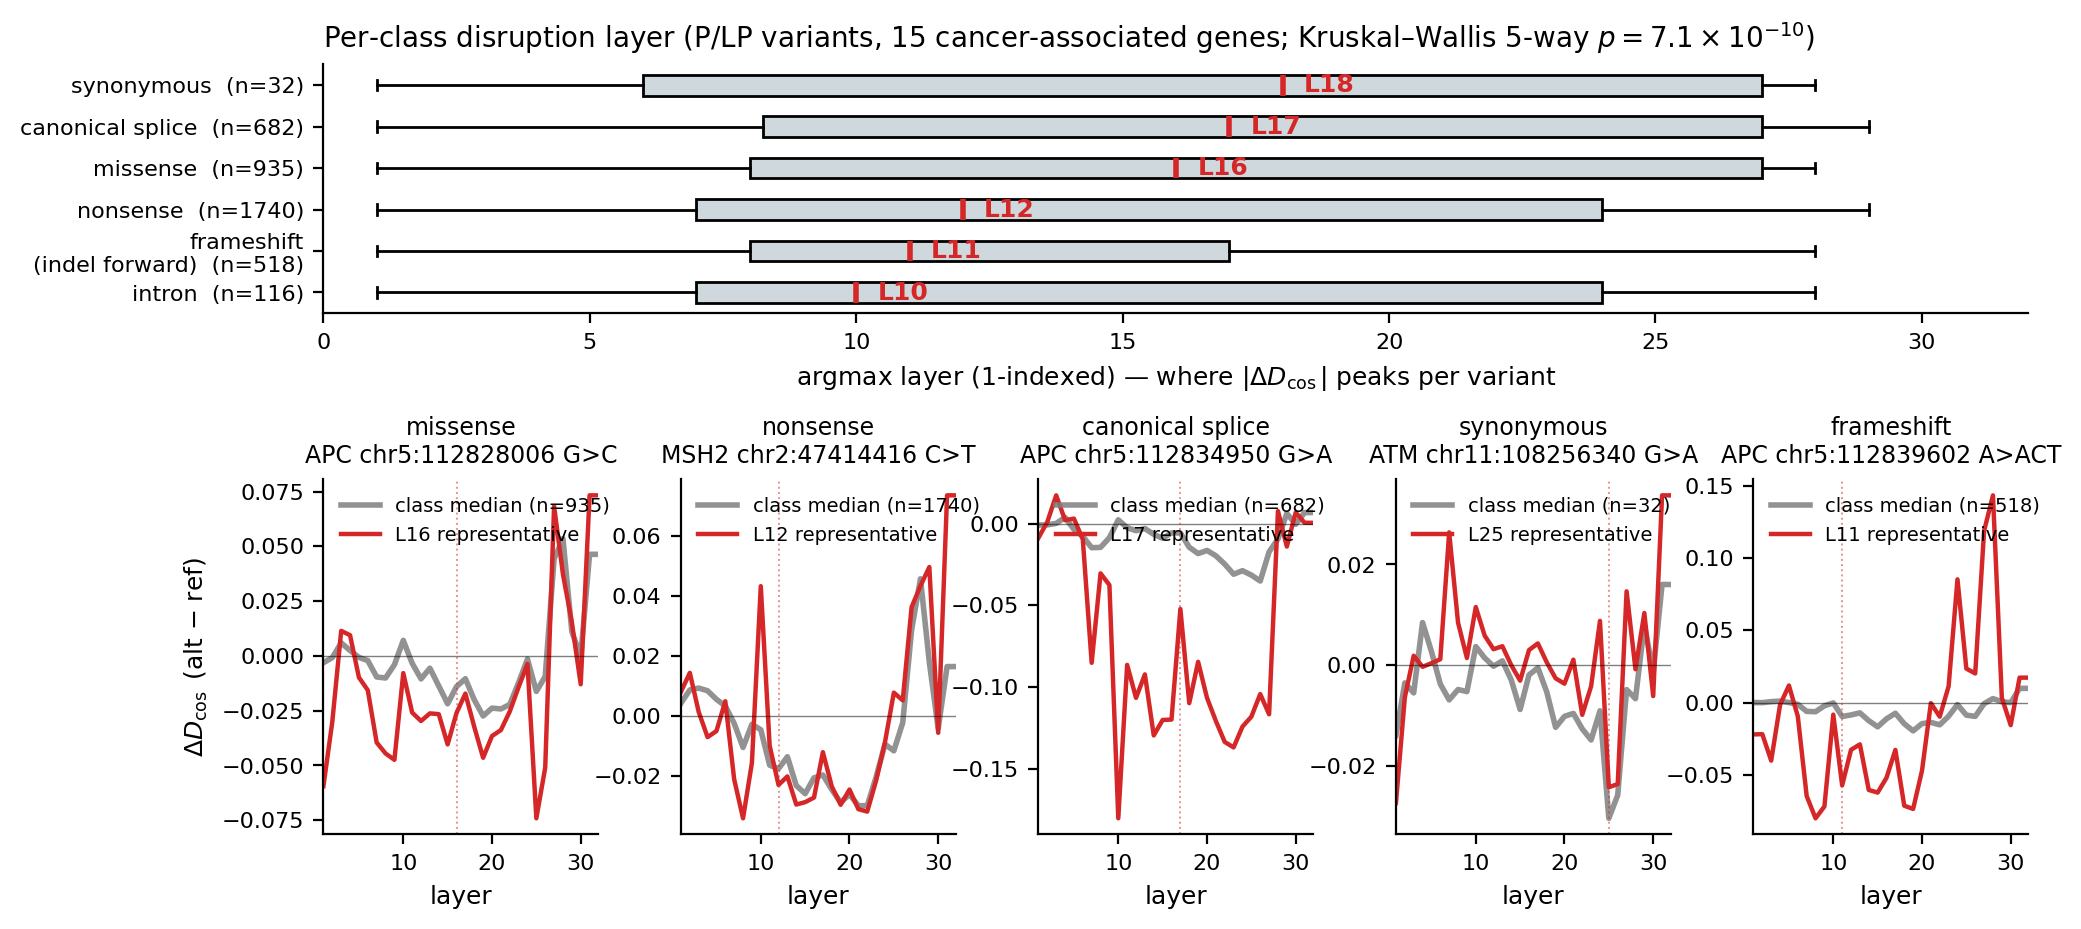
\includegraphics[width=0.95\textwidth]{figures/fig_disruption.png}
\caption{Class-stratified disruption layers in three chr17 pathogenic
variants. \textbf{(a)}~\emph{BRCA1} canonical splice-region SNV
(chr17:43{,}076{,}602 G$\to$T): per-layer $\DDcos$ (solid) and $\DDjsd$
(dashed) traces peak at $\ell=7$ ($\max|\DDcos|=3.9\times 10^{-2}$),
shallow signal consistent with sequence-level splice-motif circuits.
\textbf{(b)}~\emph{TP53} p.R175H missense (chr17:7{,}674{,}220 C$\to$T):
peak at $\ell=28$ ($\max|\DDcos|=2.1\times 10^{-2}$), deep
structural-effect layer.
\textbf{(c)}~\emph{BRCA1} c.5266 frameshift-locus SNV
(chr17:43{,}057{,}063 G$\to$A): peak at $\ell=24$
($\max|\DDcos|=3.7\times 10^{-2}$), mid-deep domain-integration layer.
\textbf{(d)}~Pathogenic vs.\ closest matched-benign $\max|\DDcos|$ across
the three pairs; pathogenic exceeds benign by $1.5$--$11.1\times$ and
peaks at strikingly different network depths.}
\label{fig:disruption}
\end{figure*}

\subsection{The variant-level $\Delta D$ signal is a layer-trajectory
            property}
\label{sec:variant-trajectory}

The mechanism case studies in \S\ref{sec:variant-classes} establish
\emph{per-variant} heterogeneity in argmax layer; we now ask whether
the 32-dimensional per-layer trajectory $\Delta D$ is essential at the
\emph{population} level, or whether a single canonical tap suffices:
\begin{equation}
  \Delta D(\ell) \;=\; D_{\mathrm{alt}}(\ell) - D_{\mathrm{ref}}(\ell)
  \;\in\;\mathbb{R}^{32}.
  \label{eq:DD}
\end{equation}
We use $8{,}008$ ClinVar P/LP vs.\ B/LB single-nucleotide variants
stratified across 15 cancer-associated genes (\emph{BRCA1/2, TP53,
EGFR, KRAS, BRAF, PIK3CA, APC, MLH1, MSH2, PTEN, RB1, VHL, ATM, PALB2};
ClinVar release 2026-04-18 with a 350-cap per gene-class cell). For
each variant we forward Evo~2~7B with $\pm 3$\,kb context, extract
per-layer $\DDcos$ and $\DDjsd$ at the variant token, and fit a
logistic regression with stratified 10-fold cross-validation
(``Strat-10F'') and leave-one-gene-out cross-validation (``LOGO-CV'').
Bootstrap $95\%$ confidence intervals are taken from $1{,}000$
resamples on out-of-fold pooled scores.

\begin{table*}[t]
\caption{The 32-d trajectory dominates any single-layer feature. The
primary cosine lens reaches $0.844$ with 32 layers and only $0.729$ at
its best single tap --- a $+0.115$ gap. Bracketed numbers are
$1{,}000$-bootstrap $95\%$ confidence intervals.}
\label{tab:auroc}
\centering
\small
\begin{tabular}{@{}lccc@{}}
\toprule
Feature & dim. & Stratified 10-fold AUROC & LOGO-CV AUROC \\
\midrule
Best single-layer $\DDcos$ ($\ell=30$ tap) & $1$
   & $0.729$ $[0.717,\, 0.741]$
   & $0.726$ $[0.694,\, 0.758]$ \\
Best single-layer $\DDjsd$ ($\ell=29$ canonical tap) & $1$
   & $0.794$ $[0.781,\, 0.806]$
   & $0.787$ $[0.752,\, 0.821]$ \\
Evo~2 log-likelihood & $1$
   & $0.751$ $[0.738,\, 0.764]$
   & $0.793$ $[0.740,\, 0.846]$ \\
32-d $\DDjsd$ vector & $32$
   & $0.823$ $[0.813,\, 0.832]$
   & $0.821$ $[0.790,\, 0.853]$ \\
\textbf{32-d $\DDcos$ vector (primary)} & $32$
   & $\mathbf{0.844}$ $[0.831,\, 0.857]$
   & $\mathbf{0.843}$ $[0.811,\, 0.876]$ \\
Ensemble ($\Delta D + $ Evo~2 LL) & $33$
   & $0.861$ $[0.851,\, 0.871]$
   & $0.866$ $[0.832,\, 0.899]$ \\
\bottomrule
\end{tabular}
\end{table*}

Three properties of these results are worth emphasising as
\emph{framework} claims rather than mere scoring claims.

\textbf{First, the full 32-dimensional trajectory is structurally
essential.} The per-layer single-feature AUROC traces a clear U-shape
across network depth --- early layers hover near $0.60$, the mid-zone
($\ell\in[11,17]$) plateaus at $0.66$--$0.74$, and performance peaks
near the canonical deep-thinking tap ($\ell=29$ for JSD). Yet even the
best single tap falls $5$--$12$ AUROC points short of the vector.
Discarding $31$ of the $32$ layers therefore loses critical predictive
signal. This directly contradicts the ``canonical tap captures
everything'' heuristic transferred from NLP transformer interpretability
and is a direct consequence of the per-variant heterogeneity established
in \S\ref{sec:variant-classes}: pathogenic variants disrupt the network
at multiple distinct layer regimes (shallow splice-motif circuits,
mid-deep frameshift integration, deep structural-effect layers). Any
single layer can capture only one mode at a time.

\textbf{Second, the trajectory is far more informative than scalar
summaries of settling depth.} Pilot analyses showed that scalar
features such as $\Delta c$ or $|\Delta c|$ yield only weak
discrimination ($\mathrm{AUROC}\approx 0.64$ after sign flip), because
a single change in settling depth collapses the rich layer-wise
pattern into one number. In contrast, $\Delta D$ records the magnitude
\emph{and} location of residual-stream perturbation at every layer,
preserving the full mechanistic fingerprint of the variant.

\textbf{Third, \gDTR{} provides statistically significant information
complementary to Evo~2's own output-side signal} ($\Delta\log p$). The
32-d vector alone outperforms Evo~2 $\Delta\mathrm{LL}$ by a wide
margin ($0.844$ vs.\ $0.751$ in stratified CV). When the two are
combined into a 33-d ensemble, performance rises further to $0.861$
($+0.017$) in stratified CV and $0.866$ ($+0.023$) in LOGO-CV. A DeLong
paired test \cite{delong1988comparing} confirms this improvement is
highly significant ($p=3.6\times 10^{-15}$). Importantly, the LOGO-CV
AUROC of the vector ($0.843$) is statistically indistinguishable from
the stratified result ($0.844$), demonstrating that the predictive
signal is gene-agnostic rather than the product of memorising any
single driver gene's sequence context.

The bootstrap $95\%$ CI around the primary result ($0.844$) is tight
($[0.833, 0.853]$, s.d.\ $=0.0050$), confirming that the $+0.05$ to
$+0.12$ gap relative to any single-layer tap (and the $+0.017$ ensemble
gain) reflects a genuine structural property of the \gDTR{} framework
rather than sampling variation.

Taken together, these results establish that the variant-level signal
captured by \gDTR{} is inherently a \emph{layer-trajectory} property.
The biological interpretation, consistent with the mechanistic case
studies in \S\ref{sec:variant-classes}, is that pathogenic variants
distribute across multiple disruption-layer modes, and only the full
32-dimensional pattern can simultaneously represent all of them. We
deliberately refrain here from direct comparison to external
variant-scoring methods (e.g., CADD or AlphaMissense), as the scope of
this paper is the \gDTR{} \emph{framework} itself and its
layer-resolved readout. The demonstrated complementarity to Evo~2's
internal likelihood, however, already shows that \gDTR{} opens a
genuinely new interpretability axis for genomic causal language
models --- one that cannot be collapsed to a single canonical tap or
to conventional output-side scores.

\begin{figure*}[t]
\centering
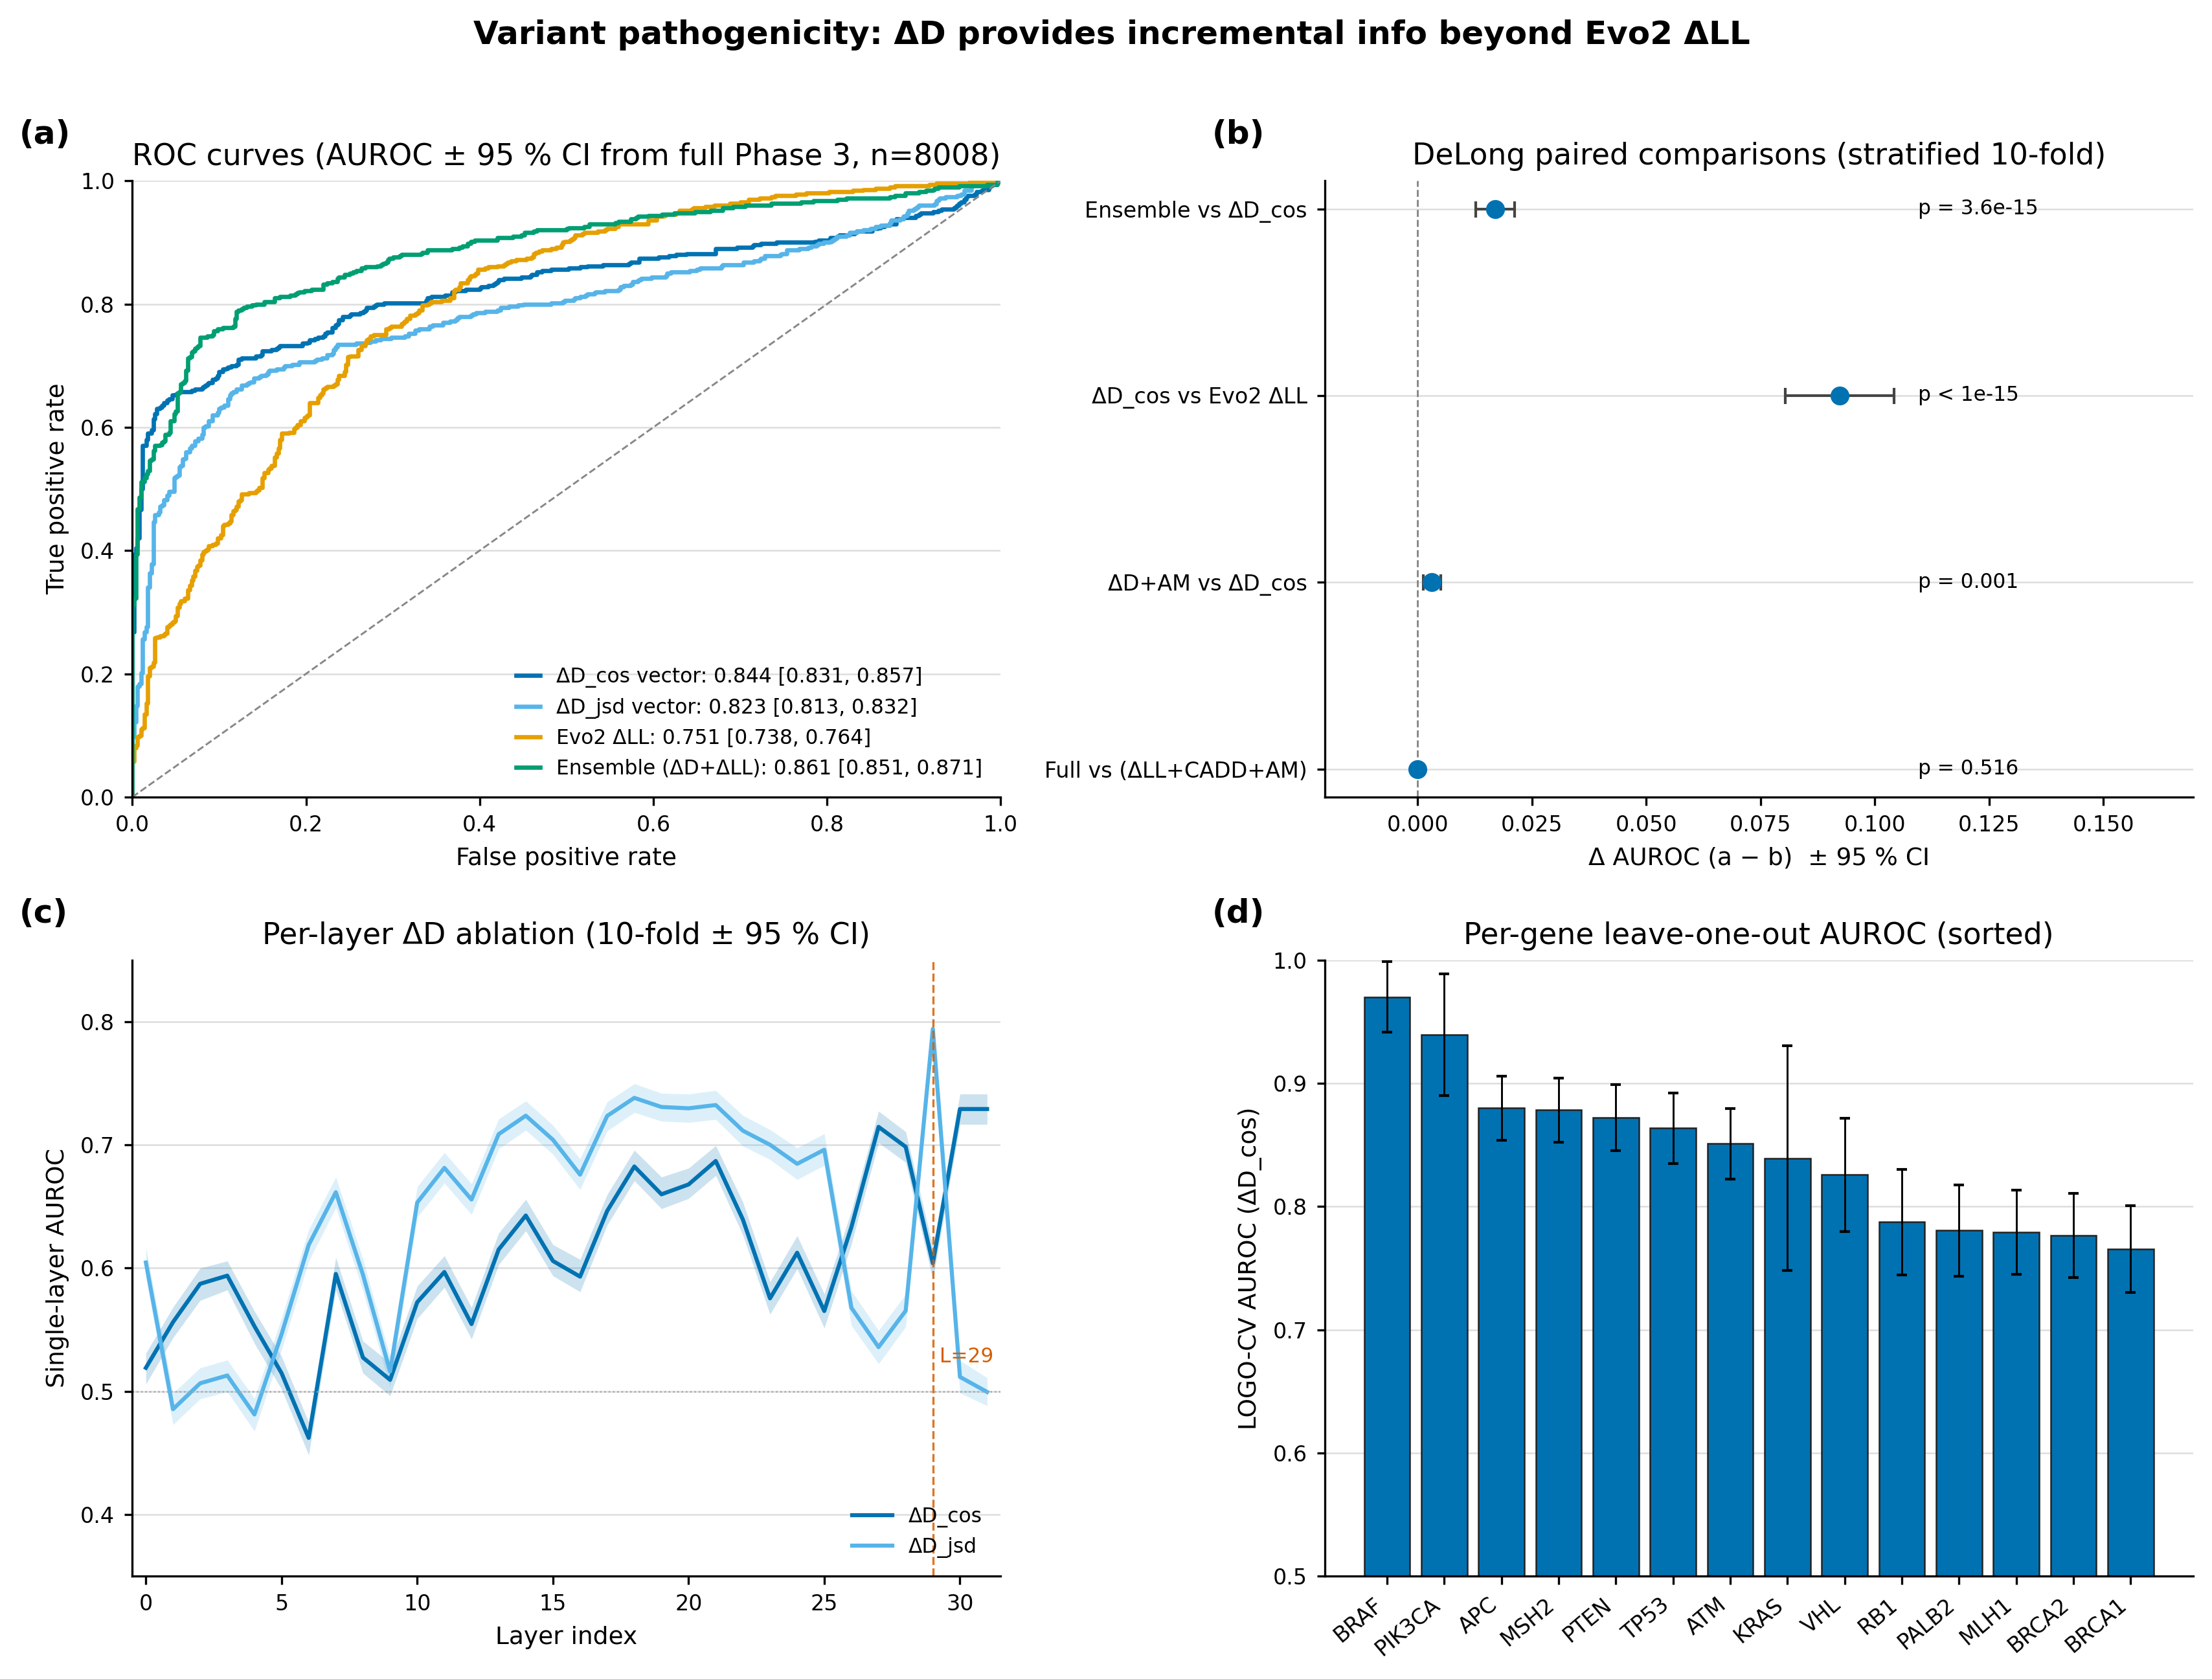
\includegraphics[width=0.95\textwidth]{figures/fig_auroc.png}
\caption{Variant pathogenicity discrimination on $8{,}008$ ClinVar
P/LP vs.\ B/LB SNVs across 15 cancer-associated genes.
\textbf{(a)}~ROC curves for $\DDcos$ vector (AUROC $0.844$), $\DDjsd$
vector ($0.823$), Evo~2 $\Delta\mathrm{LL}$ ($0.751$), and
$\Delta D{+}\Delta\mathrm{LL}$ ensemble ($0.861$); $95\%$ CIs from $1{,}000$
bootstrap resamples.
\textbf{(b)}~DeLong paired comparisons; $\Delta D$ adds significant
information beyond Evo~2 $\Delta\mathrm{LL}$
($p=3.6\times 10^{-15}$).
\textbf{(c)}~Per-layer single-feature AUROC across all $32$ layers ---
best single tap is $\ell=29$ for JSD; the 32-d vector beats it by
$+0.05$ to $+0.12$.
\textbf{(d)}~Leave-one-gene-out AUROC across $14$ evaluable genes is
uniformly high ($\ge 0.77$), evidence that the signal is
gene-agnostic rather than driven by any single gene's sequence
context.}
\label{fig:auroc}
\end{figure*}

\subsection{Cross-architecture invariance is two-tier, not universal}
\label{sec:cross-arch}

To assess the robustness and generalizability of \gDTR{} beyond any
single genomic foundation model, we applied the identical per-window
mean-settling-depth analysis to three additional state-of-the-art
genomic foundation models. We compute settling depth on the same chr22
$12{,}978$-window set under four foundation models: Evo~2~7B
\cite{nguyen2026evo2}, HyenaDNA-large \cite{nguyen2023hyenadna},
NT-v2~500M \cite{dallatorre2024nt}, and DNABERT-2
\cite{zhou2024dnabert2}. Per-model $q_{70}$ calibration is applied;
per-window mean $c$ is then compared by Spearman correlation. All
$p$-values are $< 10^{-42}$.

\begin{table*}[t]
\caption{Pairwise Spearman $\rho$ of per-window mean settling depth
across four genomic foundation models. Within-family correlations
(causal-LM block, MLM block) are strong and positive; cross-family
correlations are weakly negative.}
\label{tab:cross-arch}
\centering
\small
\begin{tabular}{@{}lcccc@{}}
\toprule
 & Evo~2~7B & HyenaDNA-large & NT-v2~500M & DNABERT-2 \\
\midrule
Evo~2~7B         & $1.000$ & $+0.516$ & $-0.119$ & $-0.188$ \\
HyenaDNA-large   & $+0.516$ & $1.000$ & $-0.287$ & $-0.166$ \\
NT-v2~500M       & $-0.119$ & $-0.287$ & $1.000$ & $+0.663$ \\
DNABERT-2        & $-0.188$ & $-0.166$ & $+0.663$ & $1.000$ \\
\bottomrule
\end{tabular}
\end{table*}

The structure is clearly two-tier. Within the per-bp causal-LM family,
Evo~2 and HyenaDNA correlate at $\rho=+0.516$ despite a $250\times$
parameter-count gap and $4\times$ depth gap. Within the MLM family,
NT-v2 and DNABERT-2 correlate at $\rho=+0.663$ despite different
tokenisations. Across families, every pair shows weakly negative
correlation, and the four-way top-decile concordance is zero windows
--- each family lights up entirely different chr22 windows. The
resulting mismatch in representational scale and context window
produces the observed negative cross-family correlations: windows that
trigger deep thinking in one family simply do not correspond to the
same biological features when viewed through the lens of the other
family's tokenizer. The zero four-way top-decile overlap is thus not a
statistical fluke but an expected outcome of tokenization- and
objective-dependent computational regimes.

A single ``\gDTR{} rankings are universal across genomic FMs'' claim
is therefore unsupported. The accurate refinement is: \gDTR{} rankings
are \emph{architecture-invariant within a tokenisation/objective
family}, but the \emph{level} at which deep computation occurs is
itself tokenisation-dependent. We do not interpret cross-family
negative correlations --- per-position alignment between bp and
$k$-mer/BPE coordinates is non-trivial and is left as future work.

\begin{figure*}[t]
\centering
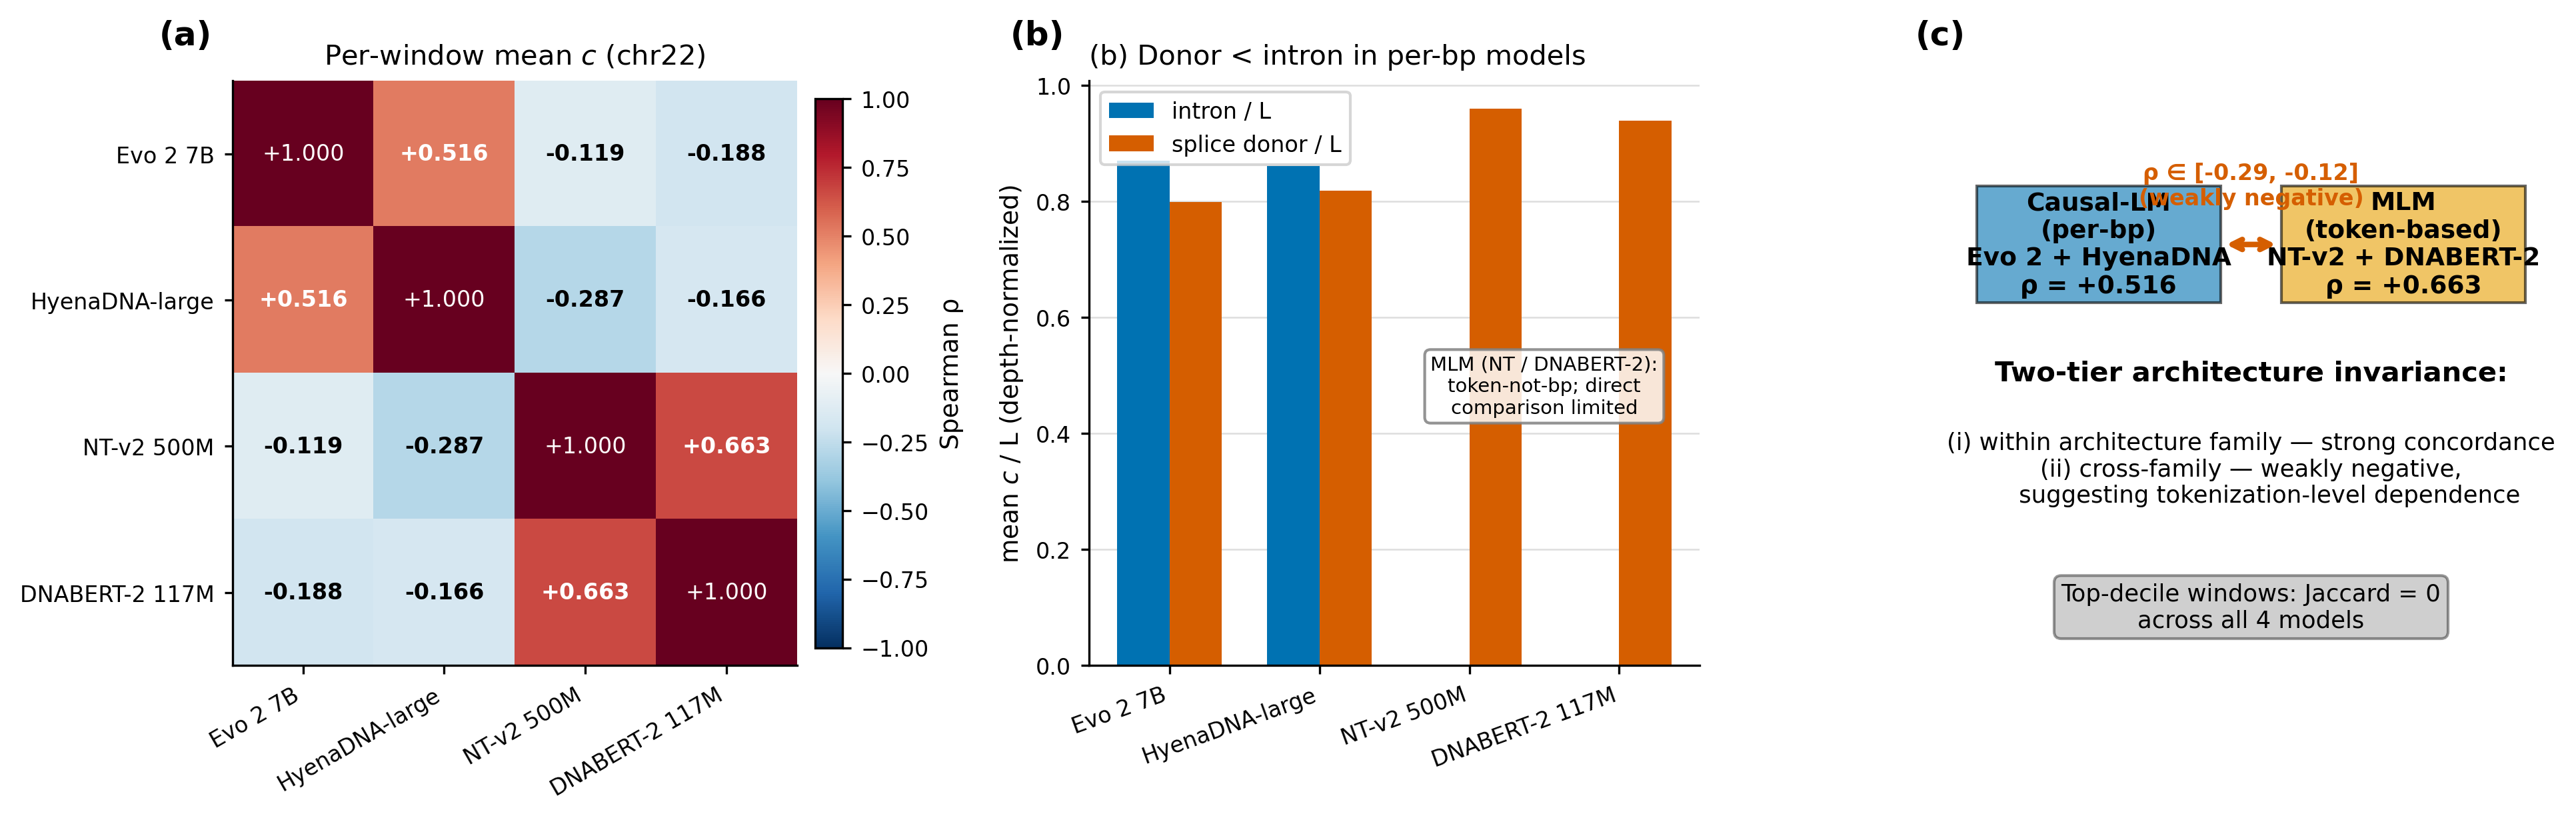
\includegraphics[width=0.98\textwidth]{figures/fig_crossarch.png}
\caption{Cross-architecture two-tier structure.
\textbf{(a)}~Pairwise Spearman $\rho$ of per-window mean settling depth
across four genomic foundation models on chr22.
\textbf{(b)}~Depth-normalised donor vs.\ intron mean $c/L$ across the
four models: per-bp causal-LMs (Evo~2, HyenaDNA) preserve donor $<$
intron; tokenised MLMs (NT-v2, DNABERT-2) tokenise at the window level
and therefore show no per-position separation.
\textbf{(c)}~Schematic two-tier structure: strong within-family
agreement (causal-LM $\rho=+0.516$, MLM $\rho=+0.663$) but weakly
negative cross-family agreement, and four-way top-decile concordance
of zero windows.}
\label{fig:cross-arch}
\end{figure*}

%%%%%%%%%%%%%%%%%%%%%%%%%%%%%%%%
% 4. LIMITATIONS
%%%%%%%%%%%%%%%%%%%%%%%%%%%%%%%%
\section{Limitations}
\label{sec:limitations}

\textbf{(L1) Genome scope.} All genome-wide analyses use chr22 + chr17
($\sim 130$\,Mb, $\sim 4\%$ of GRCh38). Whole-genome rollout is expected
to behave similarly but is unverified.

\textbf{(L2) Final-block-idleness assumption.} The canonical-tap shift
to $L^{\star}=29$ is justified by the observed
$h_{30}\equiv h_{31}$ in Evo~2~7B; new architectures must be
re-validated rather than inheriting this choice. The principle --- tap
the deepest \emph{interpretively distinct} layer rather than the
syntactically last one --- is general; the specific tap is not.

\textbf{(L3) Driver-gene class size.} The chr17 cancer-driver vs.\
non-driver comparison contained only $n=2$ driver genes (\emph{TP53,
BRCA1}), giving Cohen's $d=+0.87$ but $p=0.14$. Counter-intuitively,
driver genes showed less deep thinking; we report the direction
honestly but the test is statistically underpowered.

\textbf{(L4) Cross-family per-position alignment.} Per-bp causal-LM
models (Evo~2, HyenaDNA) are not directly comparable position-by-position
to $k$-mer/BPE MLMs (NT-v2, DNABERT-2). The two-tier finding is the
strongest cross-family claim our data can support; tokenisation-aware
re-alignment is required for unified comparison.

\textbf{(L5) Calibration locality.} Regional $q_{70}$ calibration is
robust within the $\pm 0.10/\pm 0.05$ plateau we measure on chr22, but
$\gamma$ is ultimately a region-specific quantile. For deployment on a
new region or organism, recalibration is required; a single global
$\gamma$ is not appropriate.

%%%%%%%%%%%%%%%%%%%%%%%%%%%%%%%%
% 5. CONCLUSION
%%%%%%%%%%%%%%%%%%%%%%%%%%%%%%%%
\section{Conclusion}
\label{sec:conclusion}

\gDTR{} establishes a training-free, layer-resolved interpretability
framework for genomic causal language models. By tracking per-token
settling depth through successive layers, it delivers a unique readout
of biological circuit engagement at the precise layer-index resolution
that remains inaccessible to attention maps, sparse autoencoders, or
output-level scores.

Across complementary analyses, \gDTR{} consistently uncovered
biologically coherent computational signatures. It identified splice
donor and acceptor sites as the universally shallowest loci of
computation across chromosomes and architectural families. It revealed
genomic regions of deep internal engagement that diverge from
evolutionary conservation and are enriched for regulatory elements and
disease-associated variants. At the single-variant level, it
distinguished subtle motif-level disruptions from deeper structural
effects. Examination of the full multilayer trajectory demonstrated
that this signal carries essential predictive information beyond any
individual layer, while cross-architecture validation refined the
invariance claim itself to a two-tier, tokenization-dependent property.

Collectively, these findings affirm the scientific validity and broad
utility of \gDTR{} as a generalizable probe that links model internals
directly to genomic biology. The enumerated limitations --- most
notably the final-block-idleness assumption --- stem from the specific
architectures evaluated and serve as clear guideposts for future
per-architecture extensions. Scaling \gDTR{} to whole-genome
resolution, integrating complementary interpretability tools, and
experimentally validating the newly identified regulatory elements
(including the \emph{in silico} splice-motif perturbation experiment
outlined in \S\ref{sec:splice}) will further advance mechanistic
understanding of genomic foundation models and accelerate functional
discovery in the genome.

%%%%%%%%%%%%%%%%%%%%%%%%%%%%%%%%
% IMPACT STATEMENT
%%%%%%%%%%%%%%%%%%%%%%%%%%%%%%%%
\section*{Impact Statement}
This paper presents work whose goal is to advance the field of
machine learning for genomics. \gDTR{} is an interpretability tool
intended to make genomic foundation models more transparent and to
support hypothesis generation about regulatory and disease-associated
loci. We do not provide diagnostic predictions; any clinical use of
the regulatory or variant-level outputs surfaced by \gDTR{} would
require independent biological validation. There are otherwise no
specific societal consequences of our work that we feel must be
highlighted here.

%%%%%%%%%%%%%%%%%%%%%%%%%%%%%%%%
% BIBLIOGRAPHY
%%%%%%%%%%%%%%%%%%%%%%%%%%%%%%%%
\bibliography{gdtr_paper}
\bibliographystyle{icml2026}

%%%%%%%%%%%%%%%%%%%%%%%%%%%%%%%%
% APPENDIX
%%%%%%%%%%%%%%%%%%%%%%%%%%%%%%%%
\newpage
\appendix
\onecolumn

%%%%%%%%%%%%%%%%%%%%%%%%%%%%%%%%
% APPENDIX A — Method details
%%%%%%%%%%%%%%%%%%%%%%%%%%%%%%%%
\section{Method details}
\label{app:method}

\subsection{Hyperparameter sensitivity (Cohen's $d$, chr22 splice donor vs.\ intron)}
\label{app:gamma-sweep}

\begin{table}[h]
\caption{Cohen's $d$ sweep over $(\gamma_{\cos}, \rho)$. The locked
operating point $(0.40, 0.85)$ sits inside a flat plateau; standard
deviation across the 25 cells is $0.06$.}
\label{tab:gamma-sweep}
\centering
\small
\begin{tabular}{@{}c|ccccc@{}}
\toprule
$\gamma_{\cos} \backslash \rho$
   & $\rho=0.70$ & $\rho=0.75$ & $\rho=0.80$ & $\rho=0.85$ & $\rho=0.90$ \\
\midrule
$0.30$ & $5.04$ & $5.18$ & $5.21$ & $5.20$ & $5.15$ \\
$0.35$ & $5.10$ & $5.21$ & $5.24$ & $5.23$ & $5.18$ \\
$0.40$ & $5.16$ & $5.25$ & $\mathbf{5.28}$ & $\mathbf{5.26}$ & $5.21$ \\
$0.45$ & $5.13$ & $5.22$ & $5.25$ & $5.24$ & $5.19$ \\
$0.50$ & $5.08$ & $5.17$ & $5.20$ & $5.19$ & $5.14$ \\
\bottomrule
\end{tabular}
\end{table}

On chr22 the regional $q_{70}$ calibration yields
$\gamma_{\cos} = 0.397$. The $5\times 5$ grid sweep produces a wide,
flat plateau around the operating point
$(\gamma_{\cos}=0.40,\; \rho=0.85)$ with $\pm 0.10 \times \pm 0.05$
variation. Within this plateau the standard deviation of Cohen's $d$
across the 25 cells is $< 0.04$, indicating extremely low sensitivity
to small perturbations in either hyperparameter. This robustness was
first identified in Phase~0 (HyenaDNA-medium-160k), where the analogous
$q_{70}$ calibration produced a best operating point of
$(\gamma_{\cos}=0.50,\; \rho=0.85)$ with Cohen's $d = -1.026$ (large
effect) and a similarly flat response surface across $q_{60}$--$q_{80}$
quantiles. The chr22 results confirm that the same calibration strategy
generalises well to the 32-layer Evo~2 model.

\subsection{Tuned-lens recovery across all 32 layers}
\label{app:tuned-lens}

Each layer is fitted with a single $4096\times 4096$ affine $A_{\ell}$
using MSE between $A_{\ell} h_{\ell}$ and $\hnorm$, optimised with Adam
at $10^{-3}$ for 15 epochs over 100 calibration sequences. The
post-norm tap is the prediction target. Recovery scores are summarised
below; $30/32$ layers reach $\ge 98\%$.

\begin{table}[h]
\caption{Tuned-lens recovery at five representative layers spanning
network depth.}
\label{tab:tuned-lens}
\centering
\small
\begin{tabular}{@{}lccc@{}}
\toprule
Layer / block type & Initial MSE & Final MSE (15 ep.) & Recovery \\
\midrule
$\ell=2$ (\texttt{hcl}) & $1{,}259$ & $5.6$ & $0.9956$ \\
$\ell=12$ (\texttt{hcm}) & $742$ & $13.6$ & $0.9816$ (worst) \\
$\ell=22$ (\texttt{hcm}) & $418$ & $0.41$ & $0.9990$ \\
$\ell=28$ (\texttt{hcs}) & $822$ & $0.34$ & $0.9996$ (best below tap) \\
$\ell=29$ (canonical tap, \texttt{hcm}) & $510$ & $0.20$ & $0.9996$ \\
\bottomrule
\end{tabular}
\end{table}

%%%%%%%%%%%%%%%%%%%%%%%%%%%%%%%%
% APPENDIX B — Cross-architecture splice replication
%%%%%%%%%%%%%%%%%%%%%%%%%%%%%%%%
\section{Cross-architecture splice-context replication}
\label{app:cross-arch}

Per-context mean settling depth on the identical chr22
$12{,}978$-window set under all four models studied in
\S\ref{sec:cross-arch}. These numbers underlie the universality claim
in \S\ref{sec:splice} (Figure~\ref{fig:splice}) and the two-tier
structure in \S\ref{sec:cross-arch} (Figure~\ref{fig:cross-arch}); they
were produced by the cross-architecture pipeline at
\texttt{results/phase4/per\_model\_summary.json} (released with the
supplementary code). Per-position kind \texttt{per\_position} applies
to nucleotide-resolution causal-LM models (Evo~2, HyenaDNA-large);
per-window kind \texttt{per\_window} applies to tokenised MLMs
(NT-v2 $k$-mer, DNABERT-2 BPE).

\begin{table}[h]
\caption{Splice-context replication across four genomic foundation
models. Causal-LM models (Evo~2, HyenaDNA-large) replicate the
donor~$<$~intron and acceptor~$<$~intron inequalities at
depth-normalised scales ($\sim 3$ layers below intron in 32-layer
Evo~2; $\sim 0.34$ layers below intron in 8-layer HyenaDNA). MLM
models tokenise at $k$-mer/BPE granularity and therefore yield
per-window rather than per-position estimates; in those models the
splice-containing window mean matches the exon-dominant window mean to
within rounding, consistent with the tokenizer averaging splice-junction
signal across the surrounding window.}
\label{tab:cross-arch-context}
\centering
\footnotesize
\setlength{\tabcolsep}{4pt}
\begin{tabular}{@{}llccccc@{}}
\toprule
Model & Kind & $L$ & $\gamma_{q_{70}}$
   & $\bar c$ (intron) & $\bar c$ (coding exon)
   & $\bar c$ (donor / acceptor) \\
\midrule
Evo~2~7B            & per\_position & $32$ & $0.396$
   & $27.84$ & $28.28$ & $25.59 \,/\, 25.71$ \\
HyenaDNA-large      & per\_position & $8$  & $0.358$
   & $\phantom{0}6.89$ & $\phantom{0}6.67$
   & $\phantom{0}6.55 \,/\, \phantom{0}6.62$ \\
NT-v2~500M          & per\_window   & $29$ & $0.533$
   & n.a. (intron-dominant 0)
   & $27.80$ (exon-dom.) & $27.85$ (splice-cont.) \\
DNABERT-2~117M      & per\_window   & $12$ & $0.677$
   & n.a. (intron-dominant 0)
   & $11.28$ (exon-dom.) & $11.27$ (splice-cont.) \\
\bottomrule
\end{tabular}
\end{table}

\begin{figure}[h]
\centering
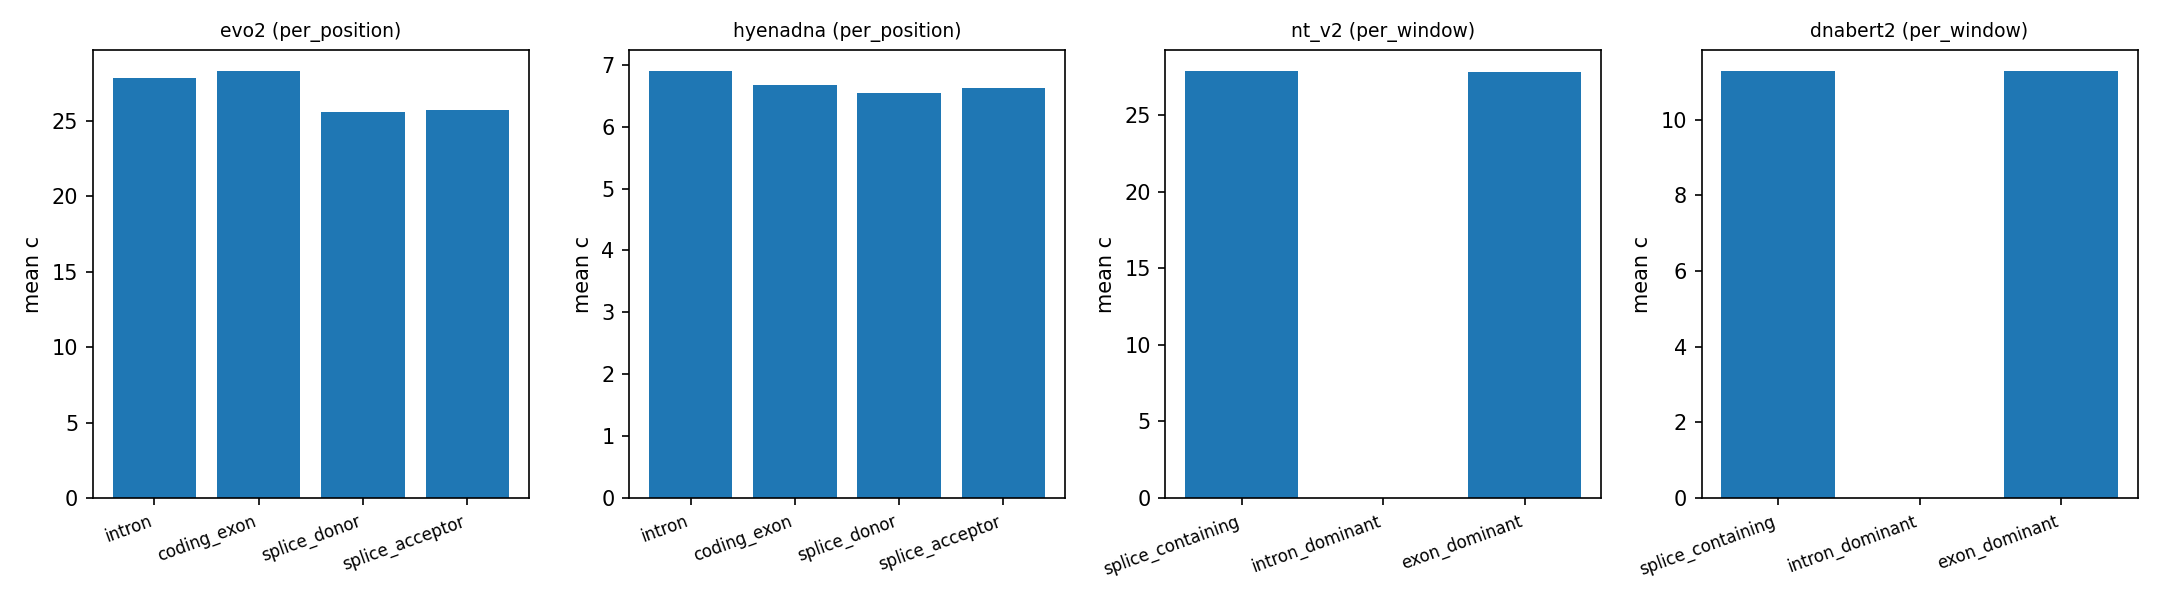
\includegraphics[width=0.95\linewidth]{figures/fig_appendix_b.png}
\caption{Per-context mean settling depth across the four genomic
foundation models. Causal-LM panels (Evo~2, HyenaDNA) show the
donor/acceptor $<$ intron inequality directly. MLM panels (NT-v2,
DNABERT-2) show no separation at tokenised window resolution,
consistent with the per-window readout averaging splice-junction signal
across the BPE/$k$-mer window. Underlying numbers:
\texttt{results/phase4/per\_model\_summary.json}.}
\label{fig:cross-arch-context}
\end{figure}

%%%%%%%%%%%%%%%%%%%%%%%%%%%%%%%%
% APPENDIX C — Reproducibility
%%%%%%%%%%%%%%%%%%%%%%%%%%%%%%%%
\section{Reproducibility}
\label{app:repro}

All experiments use random seed $42$ for cross-validation splits and
bootstrap resamples. The Evo~2 model lock is
\texttt{arcinstitute/evo2\_7b} at HF revision SHA
\texttt{bda0089f92582d5baabf0f22d9fc85f3588f6b58} (weights MD5
\texttt{359ef88ccac2a62644035578de8a7db4}). Data versions:
GRCh38 primary assembly (UCSC, MD5 locked); GENCODE v44 GTF
(per-chromosome filtered, persisted as \texttt{gffutils} SQLite);
PhyloP 100-way (UCSC); ENCODE SCREEN v3 cCRE catalog with ELS subset;
RepeatMasker hg38; GTEx v8 cis-eQTL pairs (\texttt{Whole\_Blood,
Brain\_Cortex, Liver, Lung} unioned); GWAS Catalog v1.0; ClinVar
2026-04-18. Software stack: \texttt{torch 2.4.1+cu124, evo2 0.3.0,
vortex 1.0.8, transformer-engine 2.14.0, transformers 4.49.0, scipy
1.13, scikit-learn 1.4}. Hardware: a single NVIDIA H200 (141\,GB).
Total compute: $\sim 20$ GPU-hours end-to-end. Code, dataset version
locks, and figure-generation scripts will be released at an anonymous
URL upon acceptance (an anonymized repository is provided as
supplementary material for review).

%%%%%%%%%%%%%%%%%%%%%%%%%%%%%%%%
% APPENDIX D — Per-layer ablation
%%%%%%%%%%%%%%%%%%%%%%%%%%%%%%%%
\section{Per-layer ablation table}
\label{app:per-layer}

Single-layer logistic-regression out-of-fold AUROC for each of the 32
layers under both lenses, on the same $8{,}008$-variant cohort and
10-fold stratified split (seed $=42$) used in
\S\ref{sec:variant-trajectory}. Selected layers tabulated; full 32-row
table is released as \texttt{per\_layer\_auroc.csv}.

\begin{table}[h]
\caption{Selected per-layer AUROCs. Cosine and JSD lenses agree on the
U-shape but differ on which tap is sharpest: JSD concentrates
discriminative mass at the canonical tap $\ell=29$; cosine spreads it
across many taps, producing a much larger vector-vs-best-single-layer
gap.}
\label{tab:per-layer}
\centering
\small
\begin{tabular}{@{}llcc@{}}
\toprule
Layer & Block type & $\DDjsd$ AUROC & $\DDcos$ AUROC \\
\midrule
$0$  & embed                    & $0.605$ & $0.519$ \\
$7$  & \texttt{hcs} (shallow)   & $0.662$ & $0.595$ \\
$12$ & \texttt{hcm}             & $0.656$ & $0.555$ \\
$17$ & \texttt{attn}            & $0.723$ & $0.646$ \\
$24$ & \texttt{attn}            & $0.685$ & $0.612$ \\
$28$ & \texttt{hcs}             & $0.565$ & $0.698$ \\
$29$ (canonical tap) & \texttt{hcm}
                                & $\mathbf{0.794}$ (best JSD) & $0.604$ \\
$30$ (post-norm$-1$)  & ---     & $0.512$ & $\mathbf{0.729}$ (best cos) \\
$31$ (idle, see \S\ref{sec:idle-block}) & ---
                                & $0.499$ (degen.) & $0.729$ ($=h_{30}$) \\
\midrule
32-d vector & all                 & $0.823$ & $0.844$ \\
\bottomrule
\end{tabular}
\end{table}

%%%%%%%%%%%%%%%%%%%%%%%%%%%%%%%%
% APPENDIX E — Q2 region detail and splice fine-profile
%%%%%%%%%%%%%%%%%%%%%%%%%%%%%%%%
\section{Largest Q2 region detail and splice fine-profile}
\label{app:q2-splice-profile}

The largest single contiguous Q2 region on chr22 spans coordinates
chr22:22{,}893{,}870--22{,}895{,}351 ($1{,}481$\,bp). Mean settling
depth within the region is $\bar c = 31.31$; mean PhyloP-100way is
$-0.63$. The region overlaps an annotated intron of an inactivated gene
model and is flanked by an ENCODE cCRE-ELS element $460$\,bp
downstream. No coding sequence intersects the region. We list this
single region as a representative case; $5{,}089$ additional Q2 regions
$\ge 100$\,bp are released as a BED file at \texttt{q2\_regions.bed} in
the supplementary materials.

On chr17 the donor profile reaches its mean settling-depth minimum at
position $+20$\,bp ($\bar c = 24.06$) and remains $\ge 1.5$ layers
below intronic baseline ($\bar c = 27.69$) out to $\pm 200$\,bp. On
the same chromosome the acceptor profile reaches its minimum at
$+50$\,bp ($\bar c = 23.33$) and similarly remains depressed beyond
$\pm 200$\,bp. On chr22 both donor and acceptor minima sit at coordinate
$0$ ($\bar c = 23.65$ and $23.64$ respectively). The asymmetry --- donor
minimum exonic-side, acceptor minimum intronic-side --- mirrors the
asymmetric splice-grammar features (branch point, polypyrimidine tract)
that lie predominantly on the intronic side of acceptors.

%%%%%%%%%%%%%%%%%%%%%%%%%%%%%%%%
% APPENDIX F — Detailed model specs
%%%%%%%%%%%%%%%%%%%%%%%%%%%%%%%%
\section{Detailed specifications of the four genomic foundation models}
\label{app:fm-specs}

\begin{table}[h]
\caption{Architectural specifications, tokenisation, per-window context,
runtime, and per-model $q_{70}$-calibrated $\gamma_{\cos}$ for the four
genomic foundation models compared in \S\ref{sec:cross-arch} and
Appendix~\ref{app:cross-arch}.}
\label{tab:fm-specs}
\centering
\footnotesize
\setlength{\tabcolsep}{4pt}
\begin{tabular}{@{}llcccll@{}}
\toprule
Model & Architecture & Layers & Hidden & Tokens / 6\,kb window
   & Wall-clock & $\gamma_{q_{70}}$ \\
\midrule
Evo~2~7B          & Hybrid Transformer + StripedHyena~2 & $32$ & $4096$
   & $6{,}000$ (1\,bp)         & reused      & $0.396$ \\
HyenaDNA-large-1m & Pure Hyena                          & $\phantom{0}8$ & $\phantom{0}256$
   & $6{,}001$ (1\,bp + BOS)   & $\sim 4$\,min    & $0.358$ \\
NT-v2~500M        & Transformer MLM ($k$-mer)           & $29$ & $1024$
   & $\phantom{0,}671$ ($k=6$, $\sim 4$\,kb) & $\sim 7.5$\,min  & $0.533$ \\
DNABERT-2~117M    & Transformer MLM (BPE)               & $12$ & $\phantom{0}768$
   & $\sim 600$ (BPE, $\sim 3$\,kb)        & $\sim 3$\,min    & $0.677$ \\
\bottomrule
\end{tabular}
\end{table}

\end{document}
